\documentclass[border=3pt]{standalone}
% Preâmbulo compartilhado pelos diagramas TikZ da aula 11 (Localização por Grade e Monte Carlo)
\usepackage[T1]{fontenc}
\usepackage[utf8]{inputenc}
\usepackage{lmodern}
\usepackage{amsmath}
\usepackage{xcolor}
\usepackage{tikz}
\usetikzlibrary{arrows.meta,angles,quotes,decorations.pathmorphing,calc,
                positioning,shapes.geometric,shapes.misc,backgrounds,fit,
                math}

% Paleta (mesma dos SVGs originais)
\definecolor{dblue}{HTML}{2A5B8C}
\definecolor{dorange}{HTML}{B3541E}
\definecolor{dgreen}{HTML}{4A7C59}
\definecolor{dred}{HTML}{9C4B4B}
\definecolor{dcream}{HTML}{F4F1EA}
\definecolor{dshade}{HTML}{DDD7C9}

% Função gaussiana (não normalizada por padrão de escala visual)
\pgfmathdeclarefunction{gauss}{3}{%
  \pgfmathparse{1/(#3*sqrt(2*pi))*exp(-((#1-#2)^2)/(2*#3^2))}%
}

% Estilos comuns (prefixo d... para não colidir com chaves internas do pgf)
\tikzset{
  >={Stealth[length=2mm]},
  dguide/.style={gray!55, dashed, line width=0.4pt},
  daxis/.style={gray!60, line width=0.7pt, ->},
  dbody/.style={fill=black!3, draw=black!80, line width=1pt},
  dacc/.style={draw=dblue, line width=1pt},
  dlbl/.style={black!55, font=\small},
  dsub/.style={black!45, font=\footnotesize},
  dstate/.style={circle, draw=black!80, fill=dcream, line width=1pt,
                 minimum size=17mm, font=\large, inner sep=1pt},
  dobs/.style={circle, draw=black!80, fill=dshade, line width=1pt,
               minimum size=14mm, font=\large, inner sep=1pt},
  dbox/.style={rounded corners=2pt, draw=black!80, fill=dcream, line width=1pt,
               align=center, inner sep=6pt},
  dop/.style={circle, draw=black!80, fill=white, line width=1pt,
              minimum size=6mm, inner sep=0pt, font=\small},
  dtrans/.style={->, dblue, line width=1pt},
  dmeas/.style={->, dorange, line width=1pt},
  dcurve/.style={line width=1pt, dblue},
  dcurveb/.style={line width=1.4pt, dorange},
}

\begin{document}
\hyphenpenalty=10000 \exhyphenpenalty=10000 \tolerance=9999 \emergencystretch=3em
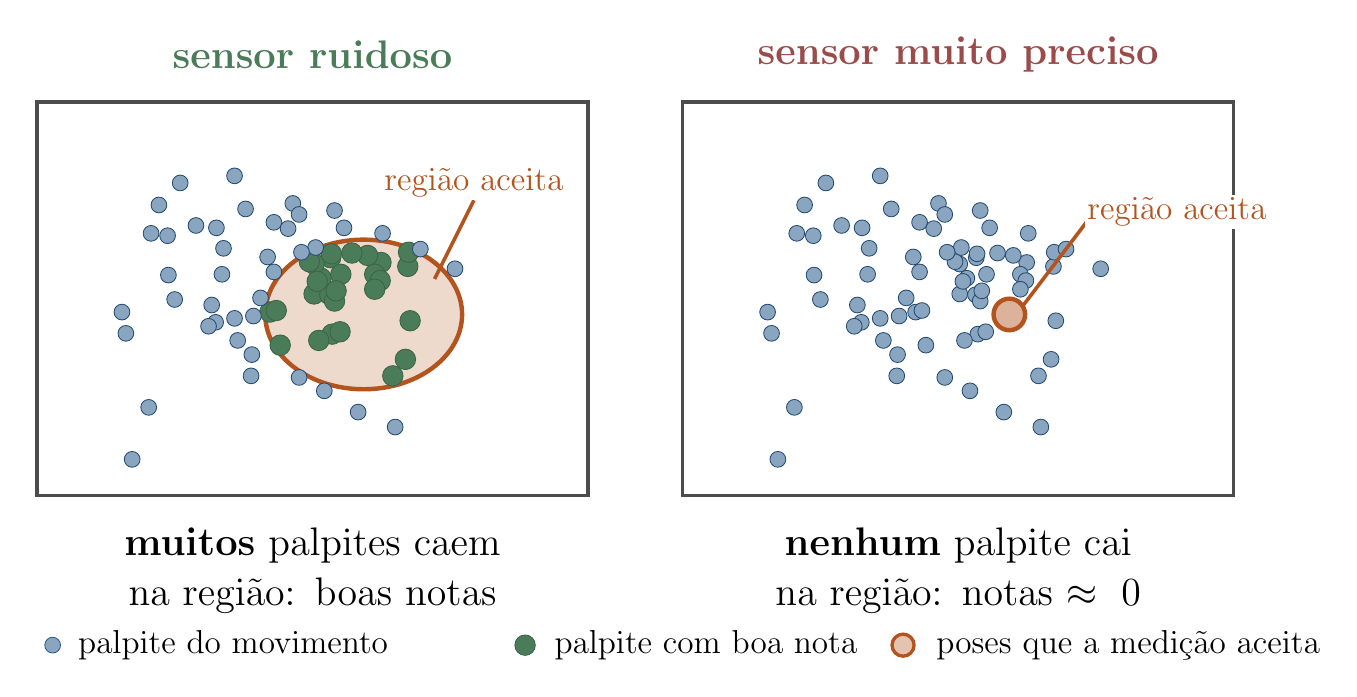
\begin{tikzpicture}[x=1cm,y=1cm]
\node[font=\Large\bfseries, dgreen] at (3.50,5.60) {sensor ruidoso};
\draw[black!70, fill=white, line width=1.2pt] (0.00,0) rectangle (7.00,5.00);
\draw[dorange, fill=dorange!22!white, line width=1.6pt] (4.15,2.30) ellipse (1.25 and 0.95);
\fill[dblue!55!white, draw=dblue!80!black, line width=0.3pt] (2.93,3.03) circle (0.10);
\fill[dgreen, draw=dgreen!80!black, line width=0.3pt] (2.96,2.33) circle (0.13);
\fill[dblue!55!white, draw=dblue!80!black, line width=0.3pt] (2.22,2.42) circle (0.10);
\fill[dgreen, draw=dgreen!80!black, line width=0.3pt] (4.37,2.96) circle (0.13);
\fill[dgreen, draw=dgreen!80!black, line width=0.3pt] (4.29,2.81) circle (0.13);
\fill[dgreen, draw=dgreen!80!black, line width=0.3pt] (3.61,2.76) circle (0.13);
\fill[dblue!55!white, draw=dblue!80!black, line width=0.3pt] (1.45,3.33) circle (0.10);
\fill[dgreen, draw=dgreen!80!black, line width=0.3pt] (3.73,3.02) circle (0.13);
\fill[dblue!55!white, draw=dblue!80!black, line width=0.3pt] (1.42,1.12) circle (0.10);
\fill[dblue!55!white, draw=dblue!80!black, line width=0.3pt] (2.27,2.20) circle (0.10);
\fill[dgreen, draw=dgreen!80!black, line width=0.3pt] (3.52,2.56) circle (0.13);
\fill[dgreen, draw=dgreen!80!black, line width=0.3pt] (3.75,2.05) circle (0.13);
\fill[dgreen, draw=dgreen!80!black, line width=0.3pt] (3.52,2.94) circle (0.13);
\fill[dblue!55!white, draw=dblue!80!black, line width=0.3pt] (2.51,4.06) circle (0.10);
\fill[dblue!55!white, draw=dblue!80!black, line width=0.3pt] (3.78,3.62) circle (0.10);
\fill[dblue!55!white, draw=dblue!80!black, line width=0.3pt] (2.55,1.97) circle (0.10);
\fill[dblue!55!white, draw=dblue!80!black, line width=0.3pt] (2.84,2.51) circle (0.10);
\fill[dgreen, draw=dgreen!80!black, line width=0.3pt] (3.86,2.81) circle (0.13);
\fill[dblue!55!white, draw=dblue!80!black, line width=0.3pt] (2.73,1.79) circle (0.10);
\fill[dblue!55!white, draw=dblue!80!black, line width=0.3pt] (2.65,3.64) circle (0.10);
\fill[dblue!55!white, draw=dblue!80!black, line width=0.3pt] (2.35,2.81) circle (0.10);
\fill[dblue!55!white, draw=dblue!80!black, line width=0.3pt] (3.65,1.33) circle (0.10);
\fill[dblue!55!white, draw=dblue!80!black, line width=0.3pt] (3.25,3.71) circle (0.10);
\fill[dblue!55!white, draw=dblue!80!black, line width=0.3pt] (1.08,2.33) circle (0.10);
\fill[dgreen, draw=dgreen!80!black, line width=0.3pt] (3.09,1.91) circle (0.13);
\fill[dgreen, draw=dgreen!80!black, line width=0.3pt] (3.72,2.55) circle (0.13);
\fill[dblue!55!white, draw=dblue!80!black, line width=0.3pt] (1.66,3.30) circle (0.10);
\fill[dblue!55!white, draw=dblue!80!black, line width=0.3pt] (3.90,3.40) circle (0.10);
\fill[dgreen, draw=dgreen!80!black, line width=0.3pt] (4.71,2.91) circle (0.13);
\fill[dblue!55!white, draw=dblue!80!black, line width=0.3pt] (3.33,1.50) circle (0.10);
\fill[dgreen, draw=dgreen!80!black, line width=0.3pt] (3.85,2.08) circle (0.13);
\fill[dblue!55!white, draw=dblue!80!black, line width=0.3pt] (2.72,1.52) circle (0.10);
\fill[dblue!55!white, draw=dblue!80!black, line width=0.3pt] (2.18,2.15) circle (0.10);
\fill[dblue!55!white, draw=dblue!80!black, line width=0.3pt] (4.55,0.87) circle (0.10);
\fill[dblue!55!white, draw=dblue!80!black, line width=0.3pt] (1.67,2.80) circle (0.10);
\fill[dgreen, draw=dgreen!80!black, line width=0.3pt] (4.72,3.09) circle (0.13);
\fill[dblue!55!white, draw=dblue!80!black, line width=0.3pt] (1.21,0.46) circle (0.10);
\fill[dgreen, draw=dgreen!80!black, line width=0.3pt] (3.58,1.97) circle (0.13);
\fill[dblue!55!white, draw=dblue!80!black, line width=0.3pt] (2.02,3.43) circle (0.10);
\fill[dgreen, draw=dgreen!80!black, line width=0.3pt] (4.36,2.73) circle (0.13);
\fill[dgreen, draw=dgreen!80!black, line width=0.3pt] (3.46,2.97) circle (0.13);
\fill[dblue!55!white, draw=dblue!80!black, line width=0.3pt] (4.87,3.13) circle (0.10);
\fill[dgreen, draw=dgreen!80!black, line width=0.3pt] (3.74,3.07) circle (0.13);
\fill[dblue!55!white, draw=dblue!80!black, line width=0.3pt] (1.55,3.69) circle (0.10);
\fill[dgreen, draw=dgreen!80!black, line width=0.3pt] (4.20,3.05) circle (0.13);
\fill[dblue!55!white, draw=dblue!80!black, line width=0.3pt] (1.13,2.06) circle (0.10);
\fill[dblue!55!white, draw=dblue!80!black, line width=0.3pt] (4.08,1.06) circle (0.10);
\fill[dblue!55!white, draw=dblue!80!black, line width=0.3pt] (3.01,3.47) circle (0.10);
\fill[dblue!55!white, draw=dblue!80!black, line width=0.3pt] (1.82,3.97) circle (0.10);
\fill[dgreen, draw=dgreen!80!black, line width=0.3pt] (3.78,2.47) circle (0.13);
\fill[dblue!55!white, draw=dblue!80!black, line width=0.3pt] (3.54,3.15) circle (0.10);
\fill[dblue!55!white, draw=dblue!80!black, line width=0.3pt] (3.33,3.57) circle (0.10);
\fill[dblue!55!white, draw=dblue!80!black, line width=0.3pt] (2.51,2.25) circle (0.10);
\fill[dgreen, draw=dgreen!80!black, line width=0.3pt] (4.29,2.62) circle (0.13);
\fill[dblue!55!white, draw=dblue!80!black, line width=0.3pt] (2.28,3.40) circle (0.10);
\fill[dgreen, draw=dgreen!80!black, line width=0.3pt] (4.74,2.22) circle (0.13);
\fill[dblue!55!white, draw=dblue!80!black, line width=0.3pt] (1.75,2.49) circle (0.10);
\fill[dgreen, draw=dgreen!80!black, line width=0.3pt] (3.04,2.35) circle (0.13);
\fill[dgreen, draw=dgreen!80!black, line width=0.3pt] (4.68,1.73) circle (0.13);
\fill[dgreen, draw=dgreen!80!black, line width=0.3pt] (4.52,1.52) circle (0.13);
\fill[dblue!55!white, draw=dblue!80!black, line width=0.3pt] (2.37,3.14) circle (0.10);
\fill[dblue!55!white, draw=dblue!80!black, line width=0.3pt] (4.39,3.33) circle (0.10);
\fill[dgreen, draw=dgreen!80!black, line width=0.3pt] (3.56,2.72) circle (0.13);
\fill[dblue!55!white, draw=dblue!80!black, line width=0.3pt] (3.36,3.09) circle (0.10);
\fill[dblue!55!white, draw=dblue!80!black, line width=0.3pt] (3.01,2.84) circle (0.10);
\fill[dgreen, draw=dgreen!80!black, line width=0.3pt] (3.80,2.60) circle (0.13);
\fill[dgreen, draw=dgreen!80!black, line width=0.3pt] (4.00,3.08) circle (0.13);
\fill[dblue!55!white, draw=dblue!80!black, line width=0.3pt] (5.31,2.88) circle (0.10);
\fill[dblue!55!white, draw=dblue!80!black, line width=0.3pt] (2.75,2.28) circle (0.10);
\fill[dblue!55!white, draw=dblue!80!black, line width=0.3pt] (3.19,3.39) circle (0.10);
\node[font=\Large, text width=7.0cm, align=center] at (3.50,-0.95) {\textbf{muitos} palpites caem na região: boas notas};
\node[font=\Large\bfseries, dred] at (11.70,5.60) {sensor muito preciso};
\draw[black!70, fill=white, line width=1.2pt] (8.20,0) rectangle (15.20,5.00);
\draw[dorange, fill=dorange!45!white, line width=1.6pt] (12.35,2.30) circle (0.2);
\fill[dblue!55!white, draw=dblue!80!black, line width=0.3pt] (11.13,3.03) circle (0.10);
\fill[dblue!55!white, draw=dblue!80!black, line width=0.3pt] (11.16,2.33) circle (0.10);
\fill[dblue!55!white, draw=dblue!80!black, line width=0.3pt] (10.42,2.42) circle (0.10);
\fill[dblue!55!white, draw=dblue!80!black, line width=0.3pt] (12.57,2.96) circle (0.10);
\fill[dblue!55!white, draw=dblue!80!black, line width=0.3pt] (12.49,2.81) circle (0.10);
\fill[dblue!55!white, draw=dblue!80!black, line width=0.3pt] (11.81,2.76) circle (0.10);
\fill[dblue!55!white, draw=dblue!80!black, line width=0.3pt] (9.65,3.33) circle (0.10);
\fill[dblue!55!white, draw=dblue!80!black, line width=0.3pt] (11.93,3.02) circle (0.10);
\fill[dblue!55!white, draw=dblue!80!black, line width=0.3pt] (9.62,1.12) circle (0.10);
\fill[dblue!55!white, draw=dblue!80!black, line width=0.3pt] (10.47,2.20) circle (0.10);
\fill[dblue!55!white, draw=dblue!80!black, line width=0.3pt] (11.72,2.56) circle (0.10);
\fill[dblue!55!white, draw=dblue!80!black, line width=0.3pt] (11.95,2.05) circle (0.10);
\fill[dblue!55!white, draw=dblue!80!black, line width=0.3pt] (11.72,2.94) circle (0.10);
\fill[dblue!55!white, draw=dblue!80!black, line width=0.3pt] (10.71,4.06) circle (0.10);
\fill[dblue!55!white, draw=dblue!80!black, line width=0.3pt] (11.98,3.62) circle (0.10);
\fill[dblue!55!white, draw=dblue!80!black, line width=0.3pt] (10.75,1.97) circle (0.10);
\fill[dblue!55!white, draw=dblue!80!black, line width=0.3pt] (11.04,2.51) circle (0.10);
\fill[dblue!55!white, draw=dblue!80!black, line width=0.3pt] (12.06,2.81) circle (0.10);
\fill[dblue!55!white, draw=dblue!80!black, line width=0.3pt] (10.93,1.79) circle (0.10);
\fill[dblue!55!white, draw=dblue!80!black, line width=0.3pt] (10.85,3.64) circle (0.10);
\fill[dblue!55!white, draw=dblue!80!black, line width=0.3pt] (10.55,2.81) circle (0.10);
\fill[dblue!55!white, draw=dblue!80!black, line width=0.3pt] (11.85,1.33) circle (0.10);
\fill[dblue!55!white, draw=dblue!80!black, line width=0.3pt] (11.45,3.71) circle (0.10);
\fill[dblue!55!white, draw=dblue!80!black, line width=0.3pt] (9.28,2.33) circle (0.10);
\fill[dblue!55!white, draw=dblue!80!black, line width=0.3pt] (11.29,1.91) circle (0.10);
\fill[dblue!55!white, draw=dblue!80!black, line width=0.3pt] (11.92,2.55) circle (0.10);
\fill[dblue!55!white, draw=dblue!80!black, line width=0.3pt] (9.86,3.30) circle (0.10);
\fill[dblue!55!white, draw=dblue!80!black, line width=0.3pt] (12.10,3.40) circle (0.10);
\fill[dblue!55!white, draw=dblue!80!black, line width=0.3pt] (12.91,2.91) circle (0.10);
\fill[dblue!55!white, draw=dblue!80!black, line width=0.3pt] (11.53,1.50) circle (0.10);
\fill[dblue!55!white, draw=dblue!80!black, line width=0.3pt] (12.05,2.08) circle (0.10);
\fill[dblue!55!white, draw=dblue!80!black, line width=0.3pt] (10.92,1.52) circle (0.10);
\fill[dblue!55!white, draw=dblue!80!black, line width=0.3pt] (10.38,2.15) circle (0.10);
\fill[dblue!55!white, draw=dblue!80!black, line width=0.3pt] (12.75,0.87) circle (0.10);
\fill[dblue!55!white, draw=dblue!80!black, line width=0.3pt] (9.87,2.80) circle (0.10);
\fill[dblue!55!white, draw=dblue!80!black, line width=0.3pt] (12.92,3.09) circle (0.10);
\fill[dblue!55!white, draw=dblue!80!black, line width=0.3pt] (9.41,0.46) circle (0.10);
\fill[dblue!55!white, draw=dblue!80!black, line width=0.3pt] (11.78,1.97) circle (0.10);
\fill[dblue!55!white, draw=dblue!80!black, line width=0.3pt] (10.22,3.43) circle (0.10);
\fill[dblue!55!white, draw=dblue!80!black, line width=0.3pt] (12.56,2.73) circle (0.10);
\fill[dblue!55!white, draw=dblue!80!black, line width=0.3pt] (11.66,2.97) circle (0.10);
\fill[dblue!55!white, draw=dblue!80!black, line width=0.3pt] (13.07,3.13) circle (0.10);
\fill[dblue!55!white, draw=dblue!80!black, line width=0.3pt] (11.94,3.07) circle (0.10);
\fill[dblue!55!white, draw=dblue!80!black, line width=0.3pt] (9.75,3.69) circle (0.10);
\fill[dblue!55!white, draw=dblue!80!black, line width=0.3pt] (12.40,3.05) circle (0.10);
\fill[dblue!55!white, draw=dblue!80!black, line width=0.3pt] (9.33,2.06) circle (0.10);
\fill[dblue!55!white, draw=dblue!80!black, line width=0.3pt] (12.28,1.06) circle (0.10);
\fill[dblue!55!white, draw=dblue!80!black, line width=0.3pt] (11.21,3.47) circle (0.10);
\fill[dblue!55!white, draw=dblue!80!black, line width=0.3pt] (10.02,3.97) circle (0.10);
\fill[dblue!55!white, draw=dblue!80!black, line width=0.3pt] (11.98,2.47) circle (0.10);
\fill[dblue!55!white, draw=dblue!80!black, line width=0.3pt] (11.74,3.15) circle (0.10);
\fill[dblue!55!white, draw=dblue!80!black, line width=0.3pt] (11.53,3.57) circle (0.10);
\fill[dblue!55!white, draw=dblue!80!black, line width=0.3pt] (10.71,2.25) circle (0.10);
\fill[dblue!55!white, draw=dblue!80!black, line width=0.3pt] (12.49,2.62) circle (0.10);
\fill[dblue!55!white, draw=dblue!80!black, line width=0.3pt] (10.48,3.40) circle (0.10);
\fill[dblue!55!white, draw=dblue!80!black, line width=0.3pt] (12.94,2.22) circle (0.10);
\fill[dblue!55!white, draw=dblue!80!black, line width=0.3pt] (9.95,2.49) circle (0.10);
\fill[dblue!55!white, draw=dblue!80!black, line width=0.3pt] (11.24,2.35) circle (0.10);
\fill[dblue!55!white, draw=dblue!80!black, line width=0.3pt] (12.88,1.73) circle (0.10);
\fill[dblue!55!white, draw=dblue!80!black, line width=0.3pt] (12.72,1.52) circle (0.10);
\fill[dblue!55!white, draw=dblue!80!black, line width=0.3pt] (10.57,3.14) circle (0.10);
\fill[dblue!55!white, draw=dblue!80!black, line width=0.3pt] (12.59,3.33) circle (0.10);
\fill[dblue!55!white, draw=dblue!80!black, line width=0.3pt] (11.76,2.72) circle (0.10);
\fill[dblue!55!white, draw=dblue!80!black, line width=0.3pt] (11.56,3.09) circle (0.10);
\fill[dblue!55!white, draw=dblue!80!black, line width=0.3pt] (11.21,2.84) circle (0.10);
\fill[dblue!55!white, draw=dblue!80!black, line width=0.3pt] (12.00,2.60) circle (0.10);
\fill[dblue!55!white, draw=dblue!80!black, line width=0.3pt] (12.20,3.08) circle (0.10);
\fill[dblue!55!white, draw=dblue!80!black, line width=0.3pt] (13.51,2.88) circle (0.10);
\fill[dblue!55!white, draw=dblue!80!black, line width=0.3pt] (10.95,2.28) circle (0.10);
\fill[dblue!55!white, draw=dblue!80!black, line width=0.3pt] (11.39,3.39) circle (0.10);
\node[font=\Large, text width=7.0cm, align=center] at (11.70,-0.95) {\textbf{nenhum} palpite cai na região: notas $\approx 0$};
\draw[dorange, line width=1.3pt] (12.53,2.42) -- (13.35,3.50);
\node[font=\large, dorange, anchor=west, fill=white, inner sep=1pt] at (13.30,3.60) {região aceita};
\draw[dorange, line width=1.3pt] (5.05,2.75) -- (5.55,3.75);
\node[font=\large, dorange, anchor=south, fill=white, inner sep=1pt] at (5.55,3.75) {região aceita};
\fill[dblue!55!white, draw=dblue, line width=0.3pt] (0.2,-1.90) circle (0.1); \node[font=\large, anchor=west] at (0.4,-1.90) {palpite do movimento};
\fill[dgreen, draw=dgreen!80!black, line width=0.3pt] (6.2,-1.90) circle (0.13); \node[font=\large, anchor=west] at (6.45,-1.90) {palpite com boa nota};
\fill[dorange!35!white, draw=dorange, line width=1.2pt] (11.0,-1.90) circle (0.14); \node[font=\large, anchor=west] at (11.3,-1.90) {poses que a medição aceita};
\end{tikzpicture}
\end{document}
